\documentclass{article}

\def\eqstart{\begin{equation}}
\def\eqend{\end{equation}}

\usepackage{graphicx} % Required for the inclusion of images
\usepackage{natbib} % Required to change bibliography style to APA
\usepackage{amsmath} % Required for some math elements 
\usepackage{geometry}
\usepackage{hyperref}

\setlength\parindent{24pt} % Removes all indentation from paragraphs

\geometry{letterpaper, portrait, margin=1in}

\renewcommand{\labelenumi}{\alph{enumi}.} % Make numbering in the enumerate environment by letter rather than number (e.g. section 6)

\usepackage{times} % Uncomment to use the Times New Roman font

%----------------------------------------------------------------------------------------
%	DOCUMENT INFORMATION
%----------------------------------------------------------------------------------------

\title{Udacity Capstone Project - Transfer Learning on Stack Exchange} % Title

\author{Kyle \textsc{Lange}} % Author name

\date{\today} % Date for the report

\begin{document}

\maketitle % Insert the title, author and date

\section{Definition}

\subsection{Project Overview}

%In this section, look to provide a high-level overview of the project in layman’s terms. Questions to ask yourself when writing this section:

%Has an overview of the project been provided, such as the problem domain, project origin, and related datasets or input data?
%Has enough background information been given so that an uninformed reader would understand the problem domain and following problem statement?

With the vast amount of knowledge and information that is available on the
internet, there is a need to accurately classify information according to its
most relevant topic so that it can be found in search queries, recommended to
users interested in that topic, etc. This problem is also found on question /
answer websites such as Stack Exchange, where one would like to be able to tag
each query with a set of relevant labels such that the query can be directed
to the appropriate person to get an answer and can be found by other users
looking for information regarding the same topic. One could also see where an
algorithm which can assign labels might be useful for say, labeling bug
tickets for a software company so that they can be automatically assigned to
the appropriate team. All of this work can be done manually, but it is tedious
and expensive. There is therefore a need to develop machine learning algorithms
which can automate much of the process.

While a supervised learning approach (with a training set of tags and queries)
would likely be one way to approach text classification problems, a different
approach would be that of transfer learning, where we train models on queries
with a completely different topic, and apply knowledge from training these
unrelated models to build a model for the queries of interest. In the case of
the \href{https://www.kaggle.com/c/transfer-learning-on-stack-exchange-tags}{Kaggle Transfer Learning on Stack Exchange competition}, we are given training
sets composed of real Stack Exchange Queries with the Title, Text, and Tags 
from six different topics and asked to predict the tags for a new topic. 

\subsection{Problem Statement}

%In this section, you will want to clearly define the problem that you are trying to solve, including the strategy (outline of tasks) you will use to achieve the desired solution. You should also thoroughly discuss what the intended solution will be for this problem. Questions to ask yourself when writing this section:

%Is the problem statement clearly defined? Will the reader understand what you are expecting to solve?
%Have you thoroughly discussed how you will attempt to solve the problem?
%Is an anticipated solution clearly defined? Will the reader understand what results you are looking for?

For this particular competition, tagged stack exchange queries are provided
for the following topics: biology, cooking, cryptography, diy
(do-it-yourself), robotics, and travel. Given these tagged queries, we are
asked to predict the tags for physics stack exchange queries. The mean F1
score (defined in Section \ref{subsec:metrics}) is used to evaluate the quality of the
model. 

The first step, since we do not know in advance what the tags are that we
would like to predict, is tag identification. To obtain the tags, the term
frequency / inverse-document frequency (tf-idf) method will be used to
identify tags which correspond to a given subject. Since each subject area has
a different number of stack exchange queries, the tf-idf scores for each
domain are scaled as if each domain had the same number of queries. What makes
this tricky is that the tags can either have one, two, three or four
words. Thus the tf-idf process will need to be repeated for different numbers
of words.

Separate threshold cutoff values are used for word tags, bigram tags,
etc. For a given threshold cutoff value \(\beta\), the threshold tf-idf value
for topic \(k\)is defined as

\eqstart
t_k = \textrm{tf-idf}_{mean,k} + \beta \textrm{tf-idf}_{stdev,k}
\eqend

where tf-idf\(_{mean,k}\) is the mean tf-idf value for a given topic and
tf-idf\(_{stdev,k}\) is the standard deviation of the tf-idf value for a topic.

That is to say, that for a given word or bigram, if the tf-idf score is
greater than \(t_k\), it is considered to be a tag. If it is less than
\(t_k\), it is not considered to be a tag. The optimum threshold
values are determined by taking a harmonic average of the f1 scores of each of
the training data sets. By doing this, this provides topics with the lowest
scores the highest weights. This prevents obtaining a solution that is only
good for specific topics.

The second step, once the tags have been identified, is to select the tags for
each physics query. Due to memory and computational constraints, a simple
approach is taken here. If a word or bigram labeled as a tag is found
in the text of a given query, the tag is assigned to that query. What is
finally submitted is a csv file with query ids and the corresponding tags that
are predicted for the query.

\subsection{Metrics}
\label{subsec:metrics}

The mean F1 score(the evaluation metric used in the Kaggle competition) will
be used to evaluate the accuracy of the model. The F1 score is a harmonic
average of precision and recall. Algorithms with high precision will produce
very few false negatives, but potentially a large number of false
positives. Conversely algorithms with high recall will produce very few false
positives, but potentially a large number of false negatives. The F1 score
penalizes very low values for either precision or recall, providing a good
balance between false positive rate and false negative rate.

The F1 score for a given query is mathematically described as

\eqstart
F1 = \frac{2 p r}{p + r},
\eqend

where \(p\) is the precision and \(r\) is the recall. These are defined as:

\eqstart
p = \frac{tp}{tp + fp}
\eqend

\eqstart
r = \frac{tp}{tp + fn}
\eqend

where \(tp\) is the number of correctly classified tags, \(fp\) is the number
of predicted tags which are incorrect, and \(fn\) is the number of true tags
which are not predicted.

As an example of how the f1 score might be calculated for an entry, suppose
a biology query has actual tags of ``human biology'', ``human anatomy'', and
``nose'' but our model predicts ``breathing'' and ``nose''.

In this case, we would have 1 true positive (``nose''), 1 false positive
(``breathing'') and 2 false negatives (``human biology'' and ``human
anatomy''). Thus our precision would be 0.5, our recall would be 0.33333, and
our f1 score would be 0.4.

The mean F1 score takes the mean of the F1 scores over each of the queries.

\section{Analysis}

\subsection{Data Exploration}

%In this section, you will be expected to analyze the data you are using for the problem. This data can either be in the form of a dataset (or datasets), input data (or input files), or even an environment. The type of data should be thoroughly described and, if possible, have basic statistics and information presented (such as discussion of input features or defining characteristics about the input or environment). Any abnormalities or interesting qualities about the data that may need to be addressed have been identified (such as features that need to be transformed or the possibility of outliers). Questions to ask yourself when writing this section:

%If a dataset is present for this problem, have you thoroughly discussed certain features about the dataset? Has a data sample been provided to the reader?
%If a dataset is present for this problem, are statistics about the dataset calculated and reported? Have any relevant results from this calculation been discussed?
%If a dataset is not present for this problem, has discussion been made about the input space or input data for your problem?
%Are there any abnormalities or characteristics about the input space or dataset that need to be addressed? (categorical variables, missing values, outliers, etc.)


The training data set is composed of stack exchange queries under the the
topics of Travel, Cooking, Cryptography, DIY (Do-it-yourself), 
Biology, and Robotics. The test data set is composed of Physics Queries with
Title and Text. The goal is to predict the tags for each physics query. No
missing data or additional fields were observed in the text. 

Some summary statistics for each of the data sets is shown in Table
\ref{tab:stats}. Overall, there is an average of 112 words per query for all
of the queries in the training and test sets. However, one can see in the
table that the number of queries differs significantly for each subject area
in the training set. Additionally, one can see that the average number of
words varies by a maximum of 62 percent and the number of tags is relatively
consistent from topic to topic, with the exception of the Travel topic, which
has one extra tag on average compared to the other topics. Note that these
summary statistics are computed after the text cleaning process described in
Section \ref{subsec:pre_process}.
 
\begin{table}[!]
\centering
\caption{Summary Statistics on Training and Test Data}
\label{tab:stats}
\begin{tabular}{|l|l|l|l|l|l|l|l|}
\hline
& Biology & Cooking & Cryptography & DIY & Robotics & Travel & Physics \\ \hline
Number of Queries & 13196  & 15404   & 10432 & 25918 & 2771 & 19279 & 81926  \\ \hline
Average number of words / query & 94 & 90 & 131 & 120 & 146 & 98 & 117 \\ \hline
Max number of words in query & 995 & 2319 & 2478 & 1623 & 2339 & 1198 & 3183 \\ \hline
Min number of words in query & 3 & 3 & 3 & 2 & 5 & 3 & 2 \\ \hline
Average number of tags / query & 2.51 & 2.31 & 2.44 & 2.28 & 2.35 & 3.39 & -
\\ \hline
\end{tabular}
\end{table}

Several selected entries are shown in Table \ref{tab:sample_data_entries}. 

\begin{table}[!]
\centering
\caption{Sample Data Entries}
\label{tab:sample_data_entries}
\begin{tabular}{|p{1.25cm}|p{0.75cm}|p{3cm}|p{7cm}|p{2cm}|}
\hline
Data Set & id & Title & Content & Tags \\ \hline
Biology & 50 & Bacterial chromatin binding data? & I'm looking for data -
maybe CHP\^2 data that shows chromatin binding to a prokaryotic genome under
some specific conditions.  Can anyone point me to a source? &
transcription, chromatin \\ \hline
Cooking & 73544 & Is it OK to mix milk and fermented dairy? & 
Some cultures believe that it's bad to mix milk and fermented dairy, like
yogurt and cottage cheese, in the same meal (as it's bad for digestion). Are
there any adverse reactions that might happen if you consume them together? & 
milk, dairy \\ \hline
Crypto & 590 & Would RSA-encrypting a private key for itself constitute a
vulnerability? & I'm planning to encrypt some individual files for storage,
using the GnuPG implementation of RSA. If I happened to encrypt the private
key corresponding to the public key used for encrypting -- either as an
internal GnuPG file or an ASCII-armored exported key -- would this constitute
a vulnerability? The key in question is password-protected, but I'd be
interested in both situations. & cryptanalysis, rsa, pgp \\ \hline
Diy & 17 & How can I hanging something on an exterior wall with vinyl siding?
& My house has vinyl siding.  If I want to hang something on an exterior wall,
can I just attach it with screws drilled through the siding?  Or do I need to
do anything to prevent water from seeping in around the screws? & vinyl-siding
\\ \hline
Robotics & 18 & What are good methods for tuning the process noise on Kalman
filters? & Most often tuning the Kalman filter noise matrices is done by trial
and error or domain knowledge. Are there more principled ways for tuning all
the Kalman filter parameters? & odometry, localization, kalman-filter \\ \hline
Travel & 31 & Sightseeing the USA by air & The next time family from overseas
comes to visit me in the USA, I would like for them to see the major sites in
the USA. Is there such a thing as a prepaid flying tour of the USA? &
air-travel, usa, sightseeing, tours \\ \hline
Physics & 32 & How to show that the Coriolis effect is irrelevant for the
whirl/vortex in the sink/bathtub? & There is a common myth that water flowing
out from a sink should rotate in direction governed by on which hemisphere we
are; this is shown false in many household experiments, but how to show it
theoretically? & - \\ \hline
\end{tabular}
\end{table}

\subsection{Exploratory Visualization}

%In this section, you will need to provide some form of visualization that summarizes or extracts a relevant characteristic or feature about the data. The visualization should adequately support the data being used. Discuss why this visualization was chosen and how it is relevant. Questions to ask yourself when writing this section:

%Have you visualized a relevant characteristic or feature about the dataset or input data?
%Is the visualization thoroughly analyzed and discussed?
%If a plot is provided, are the axes, title, and datum clearly defined?

In order to get some idea of the distribution of the number of tags that we
predict should look like, it would be helpful to look at the distribution for
the training data. Figure \ref{fig:TagCountDistribution} shows the
distribution of the number of tags for each topic area. One can see that for
most of the training topics, the distribution shows a positive skew. However,
for the travel queries, the  distribution shows a negative skew. This is
reflected in the data from Table \ref{tab:stats} where it shows that the mean
number of tags for the travel data is higher than the mean number of tags for
the other data sets. 

% histogram showing distribution of number of tags for each data set (DONE)
\begin{figure}[]
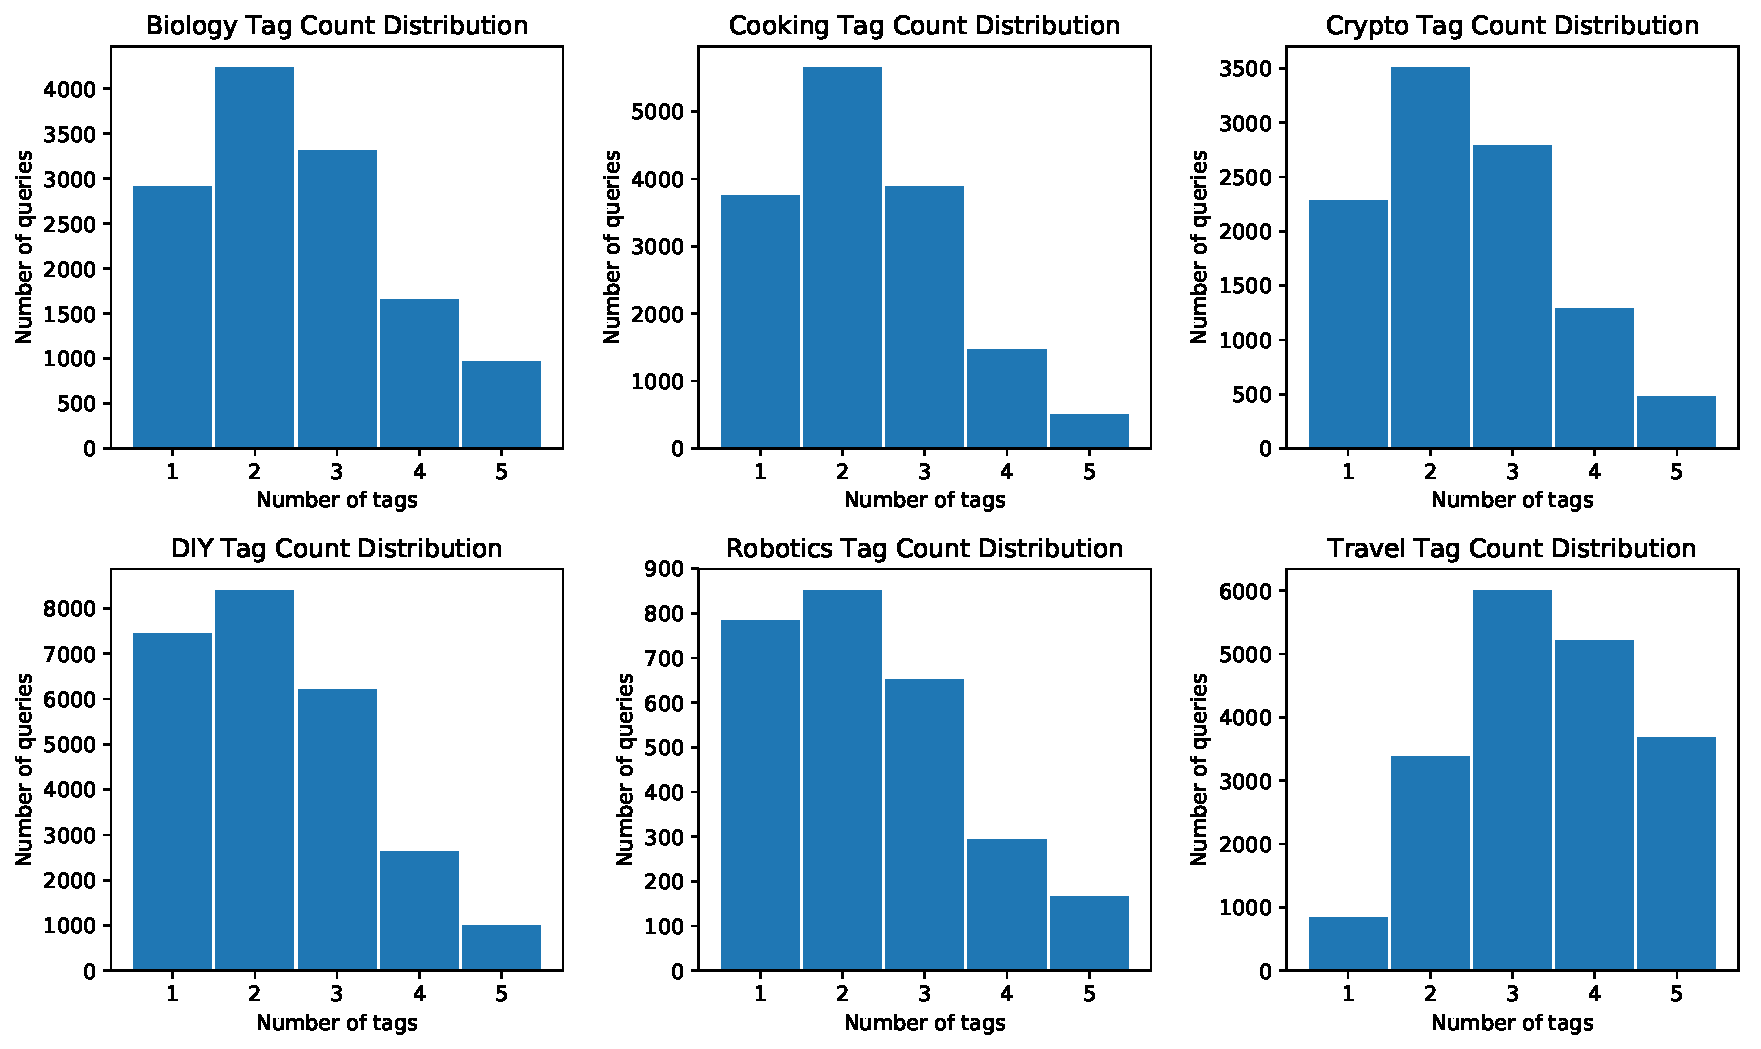
\includegraphics[width=\textwidth]{figures/TagCountDistribution.pdf}
\caption{Distribution of Number of Tags for Each Query}
\label{fig:TagCountDistribution}
\end{figure}

Given that we plan to approach the solution to this problem using a tf-idf
methodology, it would be good to see in the training data, the average number
of tags that are found in the title and content of the queries. If a large
percentage of tags are not found in the title and content of the queries, one
would expect that the success of this method would be limited. Figure
\ref{fig:PercentageFoundDistribution} shows the distribution of the number of
queries with a given percentage of the tags found in the content /
title. With the exception of the Biology queries, all of the data sets show
close to 50 percent of the tags being found in the content and title. For the
biology queries, on average, only 22 percent of the tags are actually found in
the content / title for a given query.

% plot showing percentage of entries which have tags actually in the entry /
% query (DONE)
\begin{figure}[]
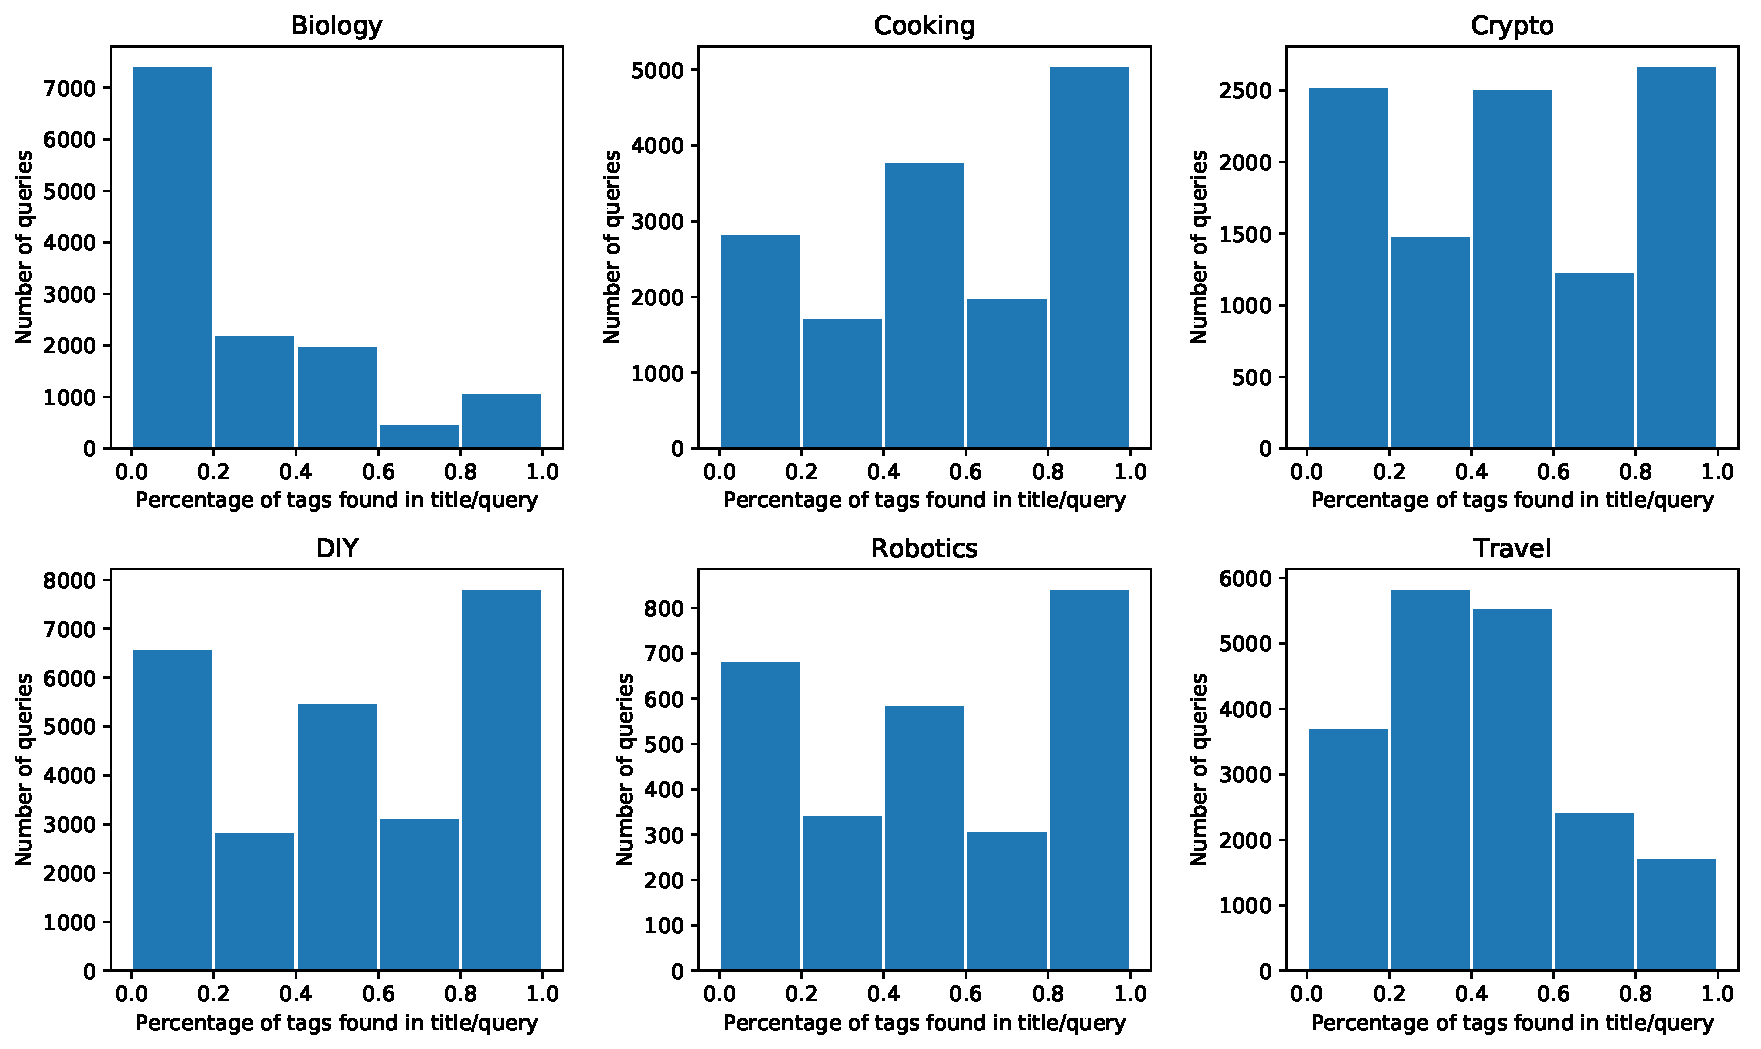
\includegraphics[width=\textwidth]{figures/PercentageFoundDistribution.pdf}
\caption{Distribution of percentage of tags actually found in content / title}
\label{fig:PercentageFoundDistribution}
\end{figure}

Given that our memory and computational requirements are limited, it would be
good to know what percentage of the tags are only word, two words, three
words, etc. Figure \ref{fig:TagWordNumberDistribution} shows the distribution
of the tags in terms of the percentage of tags having a given number of
words. Given that more than 90 percent of the tags for each data set are one
or two words and that our computational resources are limited to 4 GB of
memory, only single words and bigrams will be considered in predicting the
tags. 

% histogram showing one / two / three word tag frequencies for each subset
% (DONE)
\begin{figure}[]
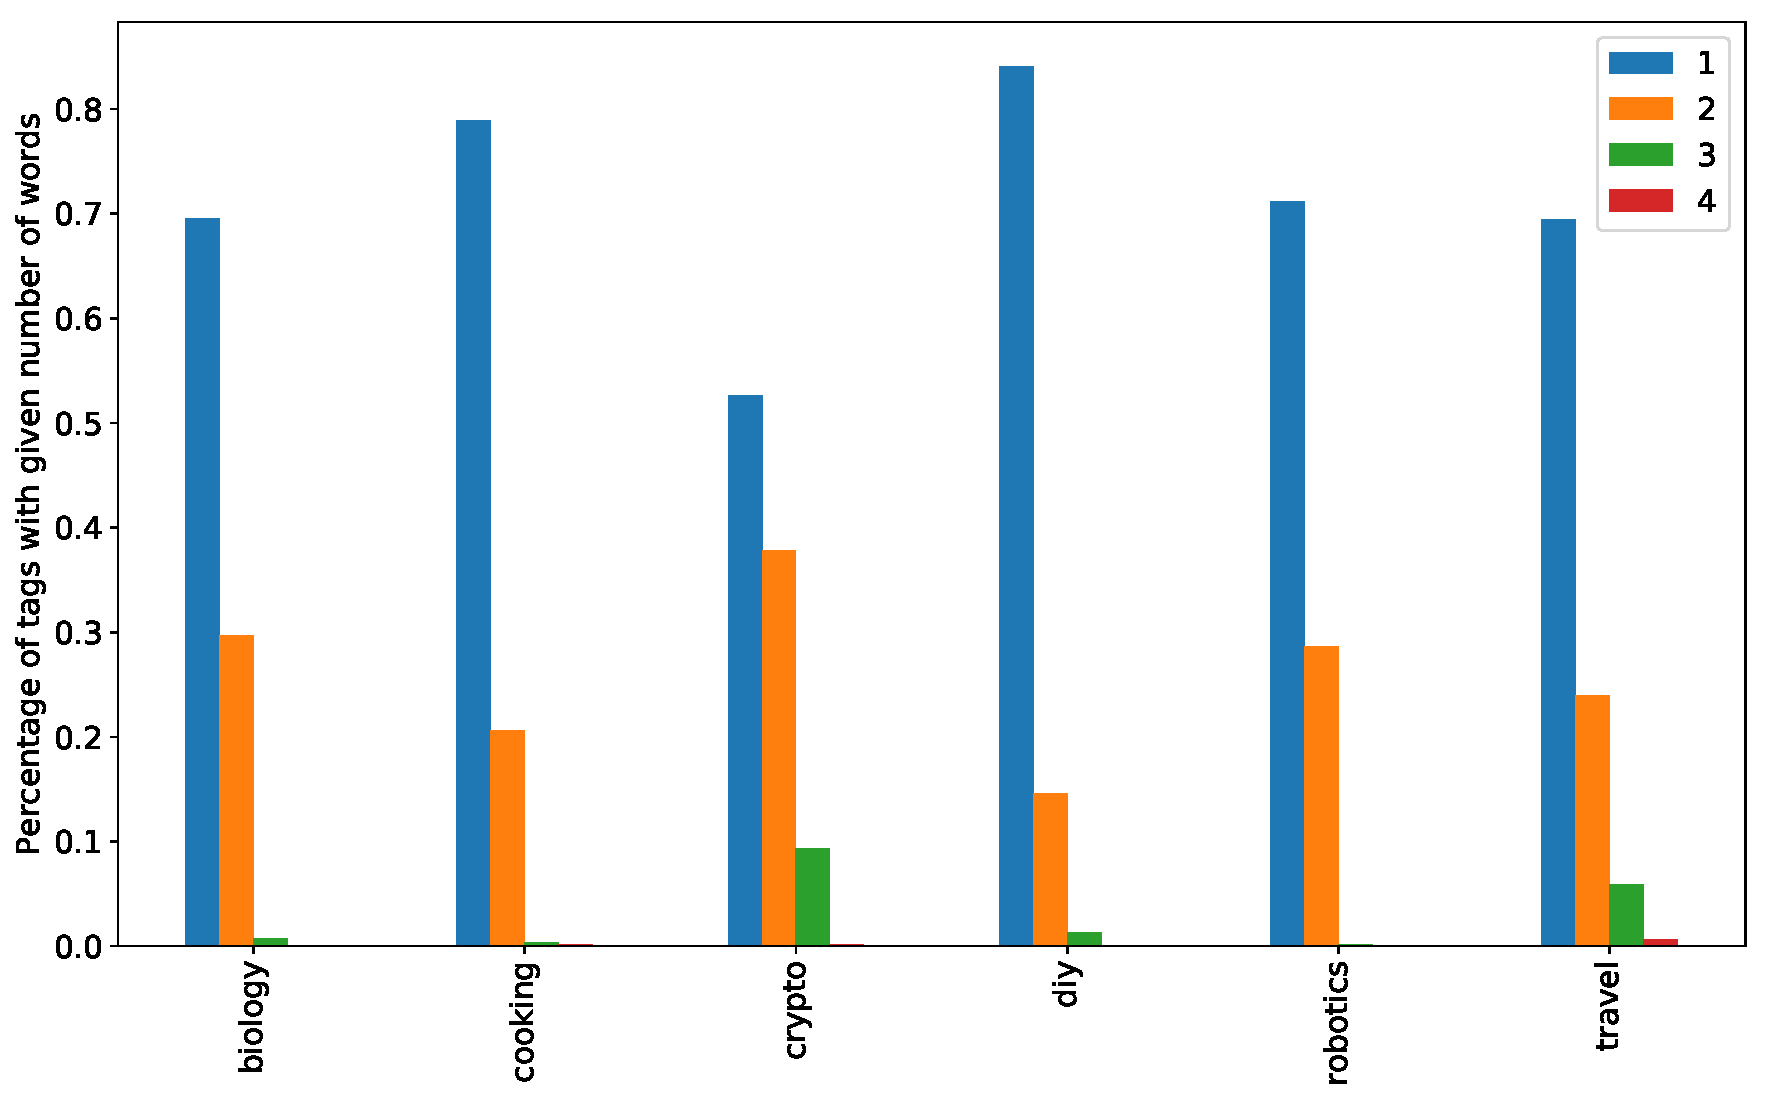
\includegraphics[width=\textwidth]{figures/TagWordNumberDistribution.pdf}
\caption{Distribution of number of words in each tag}
\label{fig:TagWordNumberDistribution}
\end{figure}



% histogram showing word count distribution (DONE)

%\begin{figure}[!]
%\label{fig:WordCountQueryDistribution}
%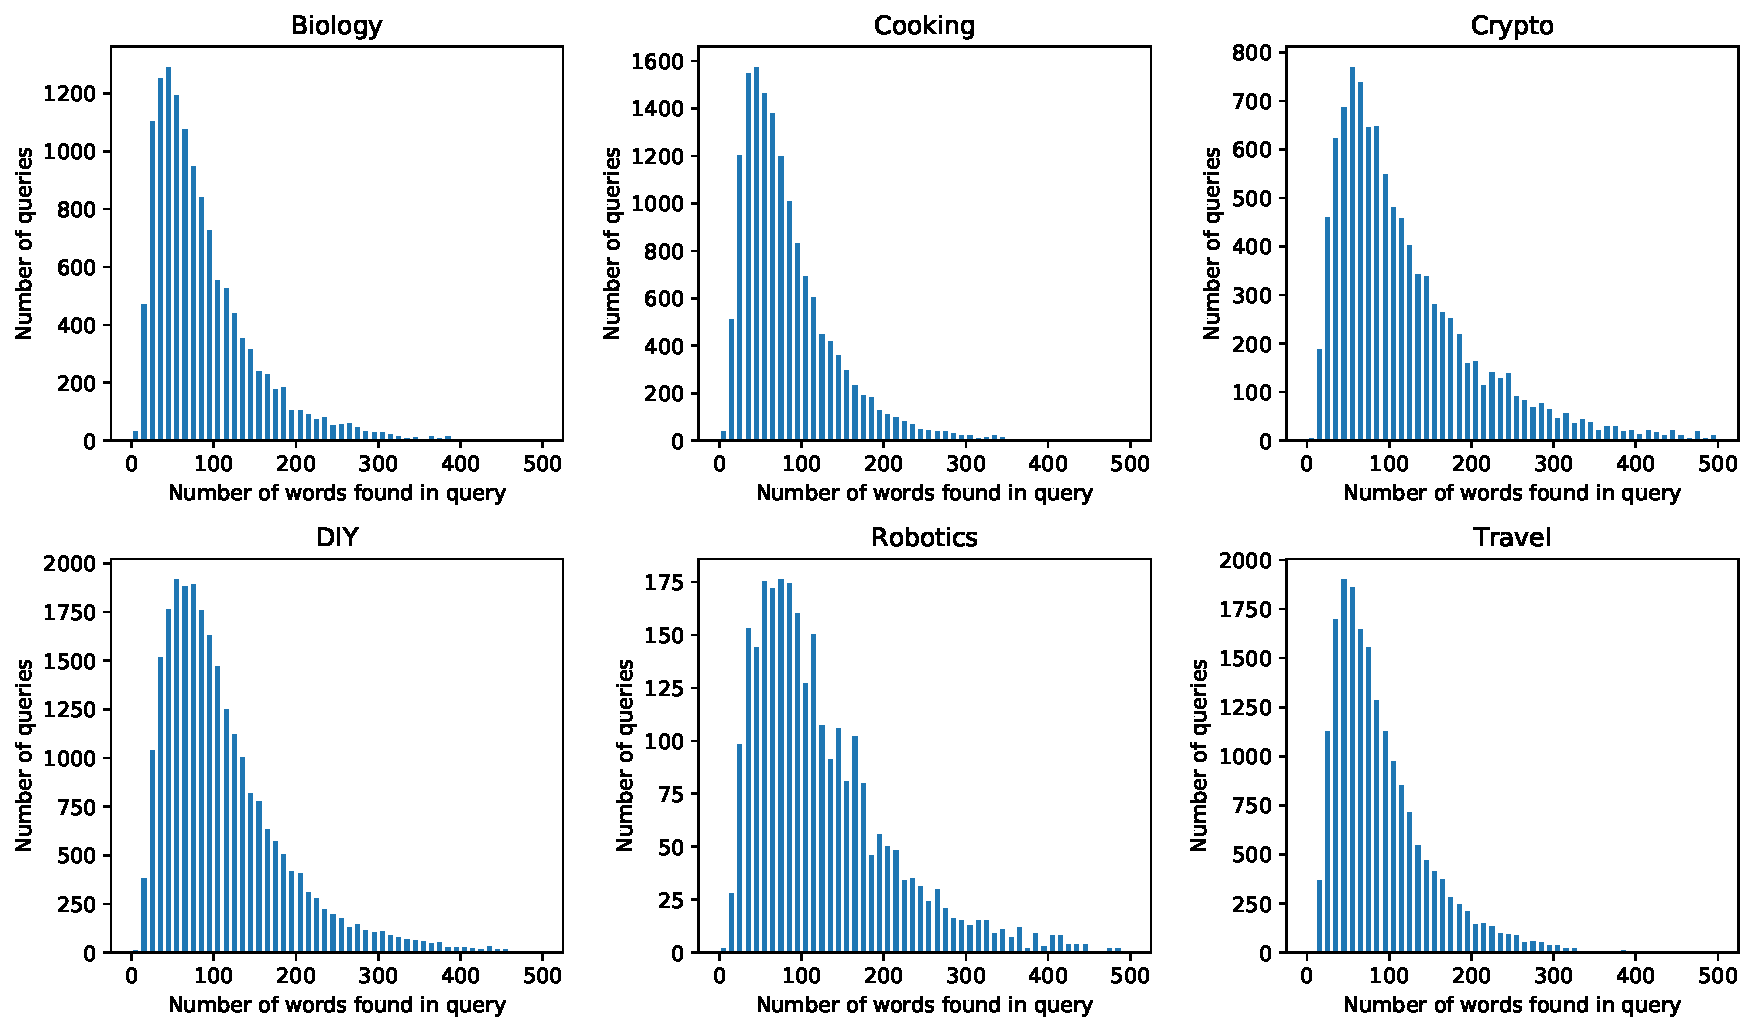
\includegraphics[width=\textwidth]{WordCountQueryDistribution.pdf}
%\caption{Distribution of number of words in content for training data}
%\end{figure}

%\begin{figure}[!]
%\label{fig:WordCountQueryTestDistribution}
%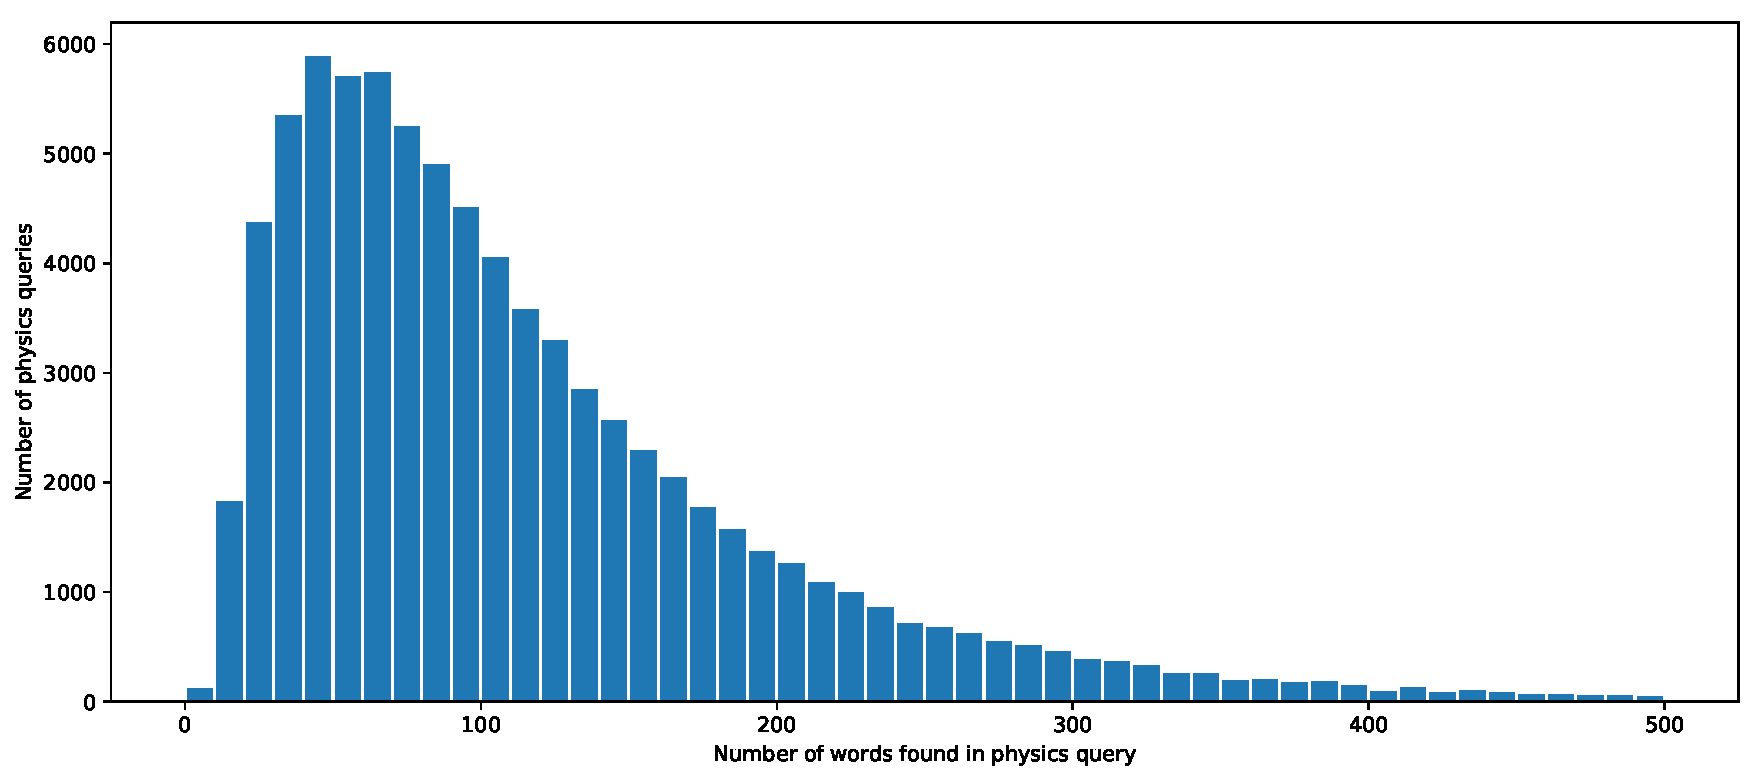
\includegraphics[width=\textwidth]{WordCountQueryTestDistribution.pdf}
%\caption{Distribution of number of words in content for test data}
%\end{figure}

\subsection{Algorithms and Techniques}

The solution to this problem is approached using two steps. The first
challenge is to identify the potential tags for the physics queries, as this
information is not known a priori. The second challenge is, given the list of
potential tags for physics queries, assign the tags to the relevant
queries. 

In order to identify the potential tags for physics queries, a variation of
the term-frequency / inverse document (tf-idf) frequency approach will be
used. The term frequency for a query \(k\) is defined to be  

\eqstart
\label{eq:tf}
tf_{t,d} = 1 + \log{f_{t,d}},
\eqend

where \(f_{t,d}\) is the number of times that a term \(t\) appears in the
content and title for a given query \(d\).

The inverse document frequency for a query \(k\) is given as

\eqstart
idf_{t} = \log{\frac{N}{n_{t}}},
\eqend

where \(N\) is the total number of queries, and \(n_{t}\) is the number of
queries containing a given term \(t\). The problem with this approach is that
the number of queries for each topic varies significantly, meaning that terms
associated with travel (19279 total queries) will occur much more frequently
than terms associated with robotics (2771 total queries). To mitigate this
problem, for the inverse document frequency, each query is inversely weighted
by the number of queries for a particular topic. 

This means that the equations for the inverse document frequency is redefined
as: 

\eqstart
\label{eq:idf}
idf_{t} = \log{\frac{N}{\sum_k \alpha_k n_{k,t}}},
\eqend

where \(n_{k,t}\) is the number of queries from topic \(k\) containing term
\(t\) and \(\alpha_k\) is defined as:

\eqstart
\alpha_k = \frac{C}{n_k},
\eqend

where \(C\) is given a constant value of 1000 and \(n_k\) is the total number
of queries for topic \(k\).

The tf-idf score for each word and bigram is computed as the product of the
term frequency and the inverse document frequency. 

Threshold values for the tf-idf scores for the bigram tags and the word tags
are specified a priori. Words and bigrams with tf-idf scores higher than their
respective threshold values are assumed to be the tags for a given topic. 

Finally, it is observed that very few of the multi-word tags contain common
words (e.g. the, a, in, and, etc.). To reduce the possibility that bigrams
will contain common words, a bigram word threshold is introduced. For each
potential bigram tag, the tf-idf score for each word is measured against a
threshold. If either word in the bigram has a tf-idf score which is below the
threshold, the bigram is thrown out and is not used as a tag.

For the second step, once the tags have been identified for the test set, the
title and content of each query are searched for each tag. All tags that are
found in the title and content of the query are assumed to be the tags for
that query.

Because the training data is different from the test data and each subset of
training data is different, standard cross-validation techniques cannot be
used. For this work, it was decided that the threshold parameters for the
tf-idf scores for words and bigrams would be determined by trying different
values for each of the six training data sets and trying to maximize the
harmonic average of the six mean f1 scores of the training data.

The harmonic average is defined to be

\eqstart
H = \frac{n}{\sum_{k=1}^{n} \frac{1}{x_k}}
\eqend

Because the mean f1 scores are not continuous when adjusting the parameters,
many optimization methods which require smooth functions and/or gradients
would not work well. For this reason, the brute force method from the scipy
optimize package was used to find the optimum parameter values which maximize
the harmonic average.

%In this section, you will need to discuss the algorithms and techniques you intend to use for solving the problem. You should justify the use of each one based on the characteristics of the problem and the problem domain. Questions to ask yourself when writing this section:

%Are the algorithms you will use, including any default variables/parameters in the project clearly defined?
%Are the techniques to be used thoroughly discussed and justified?
%Is it made clear how the input data or datasets will be handled by the algorithms and techniques chosen?


\subsection{Benchmark}

The benchmark model (provided by Kaggle) is to predict ``gravity'' as the tag
for each physics query, which results in a mean F1 score of 0.01488.  This
seems like a ``majority'' class classifier, where each query is tagged with
the most common tag; however, in this case, we don't know for certain that
this is the majority class classifier since we don't know the tags for the
physics queries. 

%In this section, you will need to provide a clearly defined benchmark result or threshold for comparing across performances obtained by your solution. The reasoning behind the benchmark (in the case where it is not an established result) should be discussed. Questions to ask yourself when writing this section:

%Has some result or value been provided that acts as a benchmark for measuring performance?
%Is it clear how this result or value was obtained (whether by data or by hypothesis)?

\section{Methodology}

\subsection{Data Preprocessing}
\label{subsec:pre_process}

The data was provided in html format in .csv files. The BeautifulSoup python
library was used to convert the html to text. All punctuation, new line
characters and words without any alphabetical characters were removed from the
content and title of each query. All of the words were converted to
lowercase. This is to make it easier to find relevant words and bigrams and to
not select numbers without any alphabetical characters as tags.

Additionally, strings starting with www and http were removed to remove direct
hyperlinks included in the text. Furthermore, due to the large number of latex
equations present in the physics data, all substrings were removed which were
enclosed between \$\$ and \$\$, \textbackslash begin \textbraceleft eq\textasteriskcentered \textbraceright and \textbackslash end\textbraceleft
eq\textasteriskcentered \textbraceright, \textbackslash
begin \textbraceleft gather \textbraceright and \textbackslash
end \textbraceleft gather \textbraceright, \textbackslash
begin \textbraceleft align \textbraceright and \textbackslash
end \textbraceleft align \textbraceright, and anything enclosed by \$
and \$, provided that one of \^{}, \textbackslash, \textbraceleft, [, ],
\textless, \textgreater, +, =, -, \textasteriskcentered, or \textunderscore
was present in the middle. 

The data preprocessing was implemented in the input\_files.py python script
and took 53-54 minutes to complete for the training and test data on my Dell
Inspiron 1300 with 4 GB of memory.

For the tags, the multi-word tags were provided with dashes between the
words. In order to avoid confusion when searching for bigram tags, all of
these dashes were removed from the tags and replaced with spaces. This was
done in the construction of the tf-idf dictionaries in tf\_idf.py.

%In this section, all of your preprocessing steps will need to be clearly documented, if any were necessary. From the previous section, any of the abnormalities or characteristics that you identified about the dataset will be addressed and corrected here. Questions to ask yourself when writing this section:

%If the algorithms chosen require preprocessing steps like feature selection or feature transformations, have they been properly documented?
%Based on the Data Exploration section, if there were abnormalities or characteristics that needed to be addressed, have they been properly corrected?
%If no preprocessing is needed, has it been made clear why?

\subsection{Implementation}

The implementation of the proposed algorithm was done using the following steps:

\begin{enumerate}
 \item Read and clean the title and content for the training data (biology,
   cooking, crypto, diy, robotics, travel) and test data (physics). All of the
   cleaned data is stored in the dataframe
 \item Construct idf python dictionaries using Eq. \ref{eq:idf} for bigrams and
   words using each of the training data sets and the test set.
  \item Loop over each training topic
  \begin{enumerate}
   \item Construct term frequency python dictionaries for bigrams and words by
     looping over each query in the training topic and applying
     Eq. \ref{eq:tf} to the words in the content and title of the query.
   \item Construct tf-idf python dictionaries for bigrams and words by
     computing the product of the tf dictionaries and the idf dictionaries.
  \end{enumerate}
 \item Loop over grid of combinations of values for word tf-idf thresholds,
   bigram tf-idf thresholds, and word bigram thresholds
 \begin{enumerate}
  \item Loop over each training topic
  \begin{enumerate}
   \item Select all words and bigrams which score above the respective
    tf-idf threshold. Additionally check bigrams to make sure that each word
    in the bigram tags has a value that is greater than the word bigram
    threshold. Designate these to be tags for the topic.
   \item Search the title and content of each query for the occurrence of any
    tags. If tags are found in a given query, the tag is assigned to the
    query.
   \item Compute the mean f1 score for the topic by comparing the predicted
    tags with the actual tags.
  \end{enumerate}
  \item Compute harmonic average of mean f1 scores for each topic. Seek to
   maximize this value using brute force optimizer.
 \end{enumerate}
 \item Once the optimum parameters have been found, repeat the process for the
   test data (physics queries) to predict the physics tags.
 \item Write out the predicted physics tags to a csv file and submit to the
   Kaggle competition.
\end{enumerate}

The tf-idf computations were implemented in the tf-idf.py file. It took
approximately 9 minutes to construct the tf-idf dictionaries after reading in
the cleaned data. The computation of the f1 score and the estimation of the
optimum parameters was done in the evaluate\_model.py file, taking
approximately 4 hours to complete. The prediction of the physics tags was
implemented in the predict\_physics\_tags.py code, taking approximately 1-2
minutes.

One of the complications that occurred during this process was that after
looking at some of the results, I noticed that the mean f1 scores were being
computed incorrectly. I had implemented the wrong function to compute the
accuracy for a given query. My function was overcounting the false positives
and as such, my accuracies were too low. After fixing this, I had to rerun the
scripts because different optimal parameter values were found. 

Note that in the capstone proposal, an additional step was proposed, in that
after tags had been predicted for the test / training data, the plan was to
look for queries which had no predicted tags, and compare the text of the
query to other queries of the same topic which have been assigned tags by
using the dot product of the tf-idf vectors of the various queries. However,
this proved to be too computationally demanding when performing the
cross-validation of the parameters and as such it was not included in the
algorithm.

%In this section, the process for which metrics, algorithms, and techniques that you implemented for the given data will need to be clearly documented. It should be abundantly clear how the implementation was carried out, and discussion should be made regarding any complications that occurred during this process. Questions to ask yourself when writing this section:

%Is it made clear how the algorithms and techniques were implemented with the given datasets or input data?
%Were there any complications with the original metrics or techniques that required changing prior to acquiring a solution?
%Was there any part of the coding process (e.g., writing complicated
%functions) that should be documented

\subsection{Refinement}

For the initial result, Table \ref{tab:initial_params} shows the values that
were chosen. This is a submission where we are allowing common words to be
used in the bigrams. We set the word bigram threshold so low that no bigrams
are discarded due to common words.

\begin{table}[!]
\centering
\caption{Initial Parameter Values}
\label{tab:initial_params}
\begin{tabular}{|l|l|}
\hline
Parameter & Value  \\ \hline
word tf-idf threshold & 2 \\ \hline
bigram tf-idf threshold & 4 \\ \hline
word bigram threshold & -100 \\ \hline
\end{tabular}
\end{table}

This resulted in a score of mean f1 score of 0.07691, good for 176th place out
of 303 teams (when the entry was submitted). While certainly a better
score than the benchmark, it is hoped that this score can be improved through
a better selection of the parameter values. 

The brute force optimization method is computationally expensive due to the
curse of dimensionality. An initial grid of parameter values is chosen as
shown in Table \ref{tab:params_sweep_values}.

\begin{table}[!]
\centering
\caption{Parameter Sweep Values}
\label{tab:params_sweep_values}
\begin{tabular}{|l|l|l|l|}
\hline
Parameter & Start Value & End Value & Interval  \\ \hline
word tf-idf threshold & 1.5 & 2.5 & 0.2 \\ \hline
bigram tf-idf threshold & 3.5 & 5.0 & 0.5 \\ \hline
word bigram threshold & -0.5 & 2.0 & 0.5 \\ \hline
\end{tabular}
\end{table}

Once the entire grid of points has been investigated, further parameter values
are chosen by the brute force optimization method near and around the value
where the maximum score was obtained. This was done using the brute force
optimization method included in the scipy library. The optimal parameters are
chosen at the point where the maximum score is found.

After running the brute force optimization, a harmonic averaged f1 mean score
of 0.165793 was obtained. The optimal parameter values are shown in Table \ref{tab:optimal_params}.

\begin{table}[!]
\centering
\caption{Optimal Parameter Values}
\label{tab:optimal_params}
\begin{tabular}{|l|l|}
\hline
Parameter & Value  \\ \hline
word tf-idf threshold & 2.126 \\ \hline
bigram tf-idf threshold & 4.395 \\ \hline
word bigram threshold & 0.496 \\ \hline
\end{tabular}
\end{table}

After submitting these to the Kaggle competition, the mean f1 score improved
to 0.08806, a 14.5 percent increase in the score from the original
result. This was good for the 101st best score out of 303 teams, an
improvement of 75 spots in the rankings.  

%In this section, you will need to discuss the process of improvement you made upon the algorithms and techniques you used in your implementation. For example, adjusting parameters for certain models to acquire improved solutions would fall under the refinement category. Your initial and final solutions should be reported, as well as any significant intermediate results as necessary. Questions to ask yourself when writing this section:

%Has an initial solution been found and clearly reported?
%Is the process of improvement clearly documented, such as what techniques were used?
%Are intermediate and final solutions clearly reported as the process is improved?

\section{Results}

\subsection{Model Evaluation and Validation}

The optimal model parameters were obtained when a harmonic averaged mean f1
score of 0.165793 was obtained for the six training categories. The breakdown
in the mean precision, mean accuracy and mean f1 score are shown in Table
\ref{tab:optimal_params_train}. One can see that the obtained mean F1 score
for the test data of 0.08806 is slightly below the range of values computed for
the various categories in the training data.

However, it is within 10 percent of the mean f1 score of the biology queries,
so it is not too concerning, especially since, in terms of the topic area,
biology and physics are both sciences and may show some similarity in their
tag properties and query structure. Finally, the physics data set is larger
than the other data sets by factors ranging from 3-30. There are probably more
physics tags than other tags, but the training data was all done on smaller
data sets. If this is true, the physics results might improve if the
thresholds are lowered further, since there would be more physics tags
relative to other data sets.

It also seems that the tf-idf method seems to favor precision over accuracy,
as the precision values are 1.7-3 times larger than the accuracy values in the
training data. This is likely due to more and more terms being considered to
be tags as the threshold gets lower. At a certain point, lowering the
threshold too much results in a situation where although more true positives
are found in the results, there are even more false positives; thus there is
little benefit to reducing the thresholds beyond this point. Thus, the model
parameters seem to be reasonable, in that they are a little on the high side,
favoring precision over accuray.

In terms of trusting the final results of this model, I would say that it
would be much better if the accuracy was improved. The model certainly
outperforms the baseline model, but ideally, to maximize the f1 score, one
would want the accuracy and the precision to have similar scores.


\begin{table}[!]
\centering
\caption{Results from Optimal Parameters}
\label{tab:optimal_params_train}
\begin{tabular}{|l|l|l|l|}
\hline
Category & Mean Accuracy & Mean Precision & Mean F1 Score  \\ \hline
Biology & 0.08049 & 0.17225 & 0.09701 \\ \hline
Cooking & 0.20431 & 0.50621 & 0.25973 \\ \hline
Cryptography & 0.13127 & 0.35155 & 0.17129 \\ \hline
DIY & 0.13603 & 0.36778 & 0.17987 \\ \hline
Robotics & 0.18585 & 0.29979 & 0.20065 \\ \hline
Travel & 0.14561 & 0.29920 & 0.17698 \\ \hline
\end{tabular}
\end{table}

In order to test the sensitivity of the model to changes in the input data, 20
percent of the records were randomly removed and the analysis was run
again. A comparison of the harmonically averaged mean f1 score and the optimal
parameter values is shown in Table \ref{tab:compare_sensitivity}. One can see
that the results were largely consistent between the two tests. The largest
change was in the word bigram threshold, which increased by 4.44 percent. All
other changes were less than 2 percent. This indicates that the model is
robust and is not overfit to the training data.

\begin{table}[!]
\centering
\caption{Sensitivity Analysis Comparison}
\label{tab:compare_sensitivity}
\begin{tabular}{|l|l|l|l|}
\hline
Output & Full Data & 80 Percent Data & Relative Change  \\ \hline
Harmonically Averaged Mean F1 score & 0.165793 & 0.167582 & 0.0108 \\ \hline
Word Threshold & 2.126 & 2.146 & 0.0094 \\ \hline
Bigram Threshold & 4.395 & 4.367 & -0.0064 \\ \hline
Word Bigram Threshold & 0.496 & 0.518 & 0.0444 \\ \hline
Test Mean F1 Score & 0.08806 & 0.08637 & -0.0192 \\ \hline
\end{tabular}
\end{table}


%In this section, the final model and any supporting qualities should be evaluated in detail. It should be clear how the final model was derived and why this model was chosen. In addition, some type of analysis should be used to validate the robustness of this model and its solution, such as manipulating the input data or environment to see how the model’s solution is affected (this is called sensitivity analysis). Questions to ask yourself when writing this section:

%Is the final model reasonable and aligning with solution expectations? Are the final parameters of the model appropriate?
%Has the final model been tested with various inputs to evaluate whether the model generalizes well to unseen data?
%Is the model robust enough for the problem? Do small perturbations (changes) in training data or the input space greatly affect the results?
%Can results found from the model be trusted?

\subsection{Justification}

Given that the benchmark mean F1 score of predicting ``gravity'' for all
entries was 0.01488 and the optimized mean F1 score was 0.08806, one can see
that a vast improvement has been made, 491 percent to be exact! It is
difficult to gain further statistics (e.g. accuracy, precision) on the
benchmark model given that I do not have access to the true solution for the
test data in the Kaggle competition.

However, the benchmark model was a simple model that could not be expected to
solve the problem. Even though the solution does far better than the
benchmark, I would say that this problem is not solved, given where the
solution places on the leaderboard and the number of factors that are not
accounted for in the model.

The model proposed here does not account for tags which are not included in
the query text; it does not take stop words into account, consider singular
/ plural forms of words, analyze word patterns to distinguish between nouns
and adjectives or do any type of clustering analysis to predict tags. I would
not say that the problem has been rigorously solved at this point.

%In this section, your model’s final solution and its results should be compared to the benchmark you established earlier in the project using some type of statistical analysis. You should also justify whether these results and the solution are significant enough to have solved the problem posed in the project. Questions to ask yourself when writing this section:

%Are the final results found stronger than the benchmark result reported earlier?
%Have you thoroughly analyzed and discussed the final solution?
%Is the final solution significant enough to have solved the problem?

\section{Conclusion}

\subsection{Free-Form Visualization}

Figure \ref{fig:training_slice} shows a slice of the results obtained during
the brute force optimization process. The harmonically averaged mean f1 score
changed very little when the word bigram threshold was changed compared to the
other parameter values. Thus, I considered a slice at the optimum word bigram
threshold value of 0.5. One can see that the results are more sensitive to
changes in the word threshold compared to changes in the bigram
threshold. One can also see that for a given word threshold, the maximum score
was found when the bigram threshold was around 

Initially as the word threshold is increased, the harmonically averaged mean
f1 score increases. However, at a certain point, around 2.3, the harmonically
averaged mean f1 score starts to decrease with corresponding increases in the
word threshold.

From looking at the plot, the solution looks rather convex, which is somewhat
surprising given the potentially discontinuous nature of the solution. Perhaps
the harmonic averaging of the mean f1 scores serves to smooth out the solution.

\begin{figure}[]
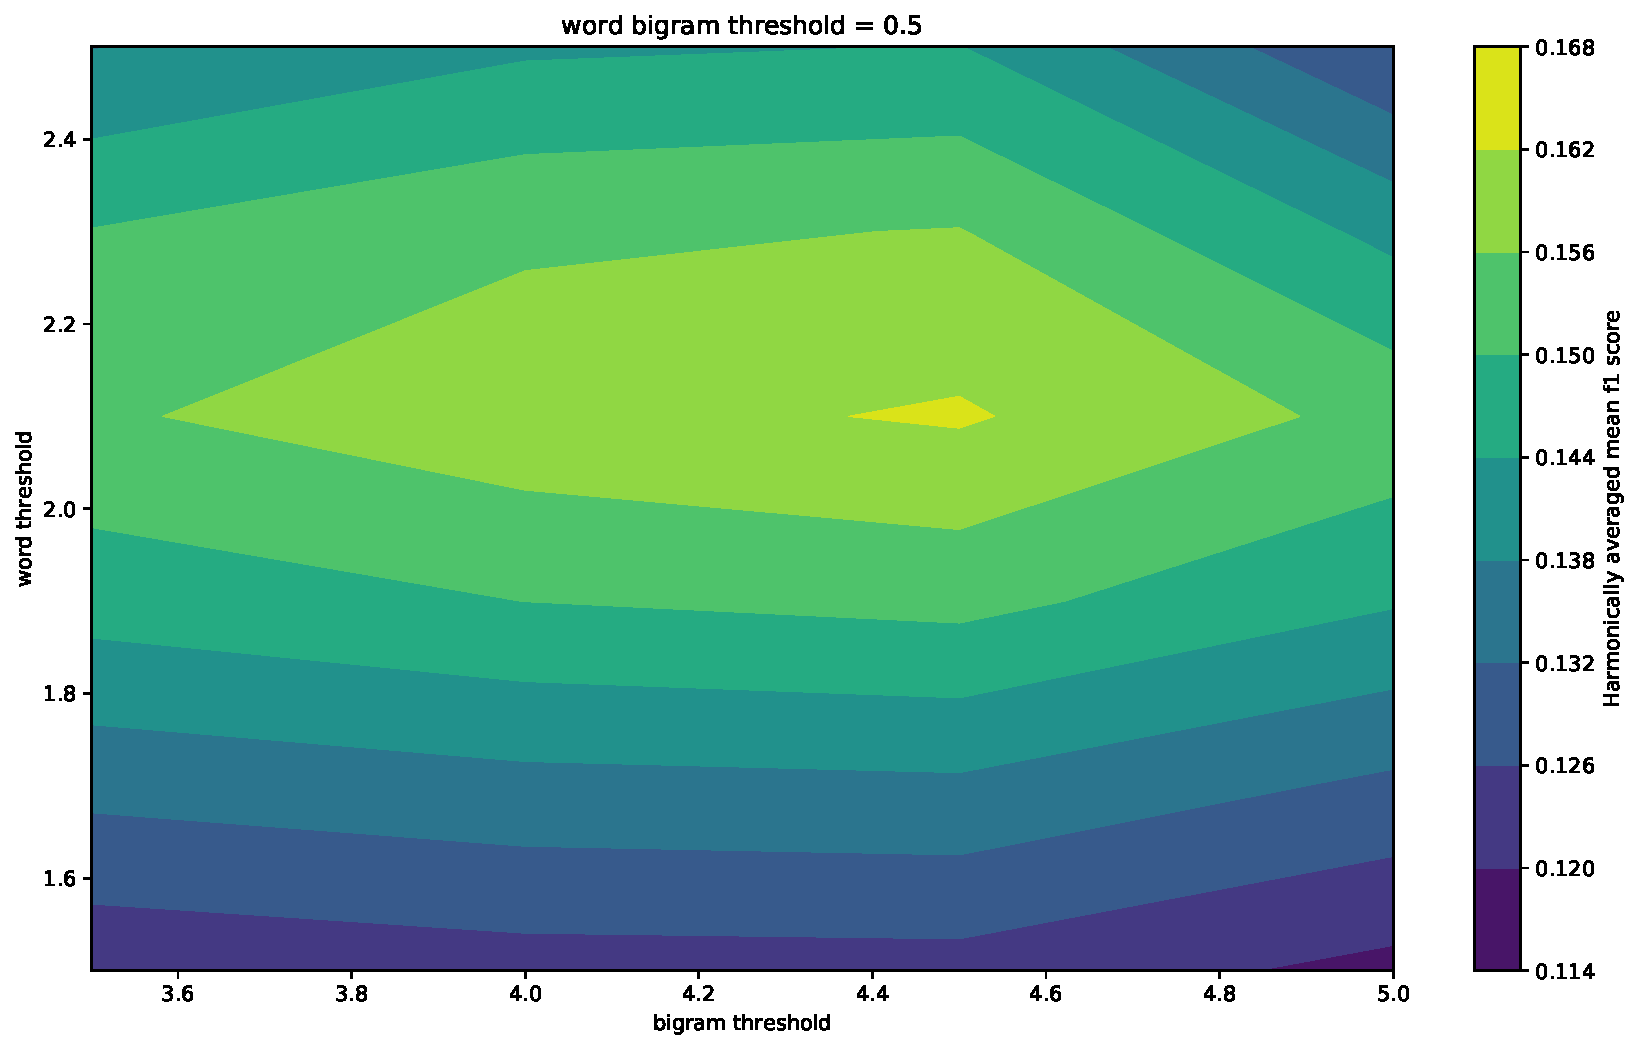
\includegraphics[width=\textwidth]{figures/OptimizationSlice.pdf}
\caption{Contour plot of brute force optimization harmonically averaged mean
  f1 scores for word bigram threshold = 0.5}
\label{fig:training_slice}
\end{figure}


%In this section, you will need to provide some form of visualization that emphasizes an important quality about the project. It is much more free-form, but should reasonably support a significant result or characteristic about the problem that you want to discuss. Questions to ask yourself when writing this section:

%Have you visualized a relevant or important quality about the problem, dataset, input data, or results?
%Is the visualization thoroughly analyzed and discussed?
%If a plot is provided, are the axes, title, and datum clearly defined?

\subsection{Reflection}

In creating this model, a number of steps were required. First, the data
needed to be cleaned: symbols removed, changed to lower-case, etc. Then the
data needed to be visualized to provide information about what one could
expect from the final solution. Next, the features needed to be created
(tf-idf scores for words and bigrams). Then, the brute force parameter
sweep needed to be completed to find the optimum model parameters. Finally,
after obtaining the optimum parameters, a prediction could be made for the
test data.

One particular part of the project which was interesting / challenging for me
was the cleaning of the data. It took a lot more time than I expected and I
had to learn about using regular expressions in python, which I didn't know
much about. Even the regular expressions that were used to clean the data
could probably be made more efficient.

Another challenging part of the project was the accurate computation of the
tf-idf scores. When computing the inverse document frequency, one had to be
very careful not to double count words or bigrams that appeared multiple times
in one query. It was necessary to insert new entries into the dictionary when
a word or bigram was in the dictionary, but when they were in the dictionary,
only the count needed to be incremented by a constant value.

I would say that the final model and solution fit my expectations for the
problem. I would not recommend this as a final solution as there are other
algorithms (e.g. RAKE) which have been mentioned in the Kaggle forums and have
been shown to obtain much higher mean f1 scores than what I obtained. However,
it is a good starting point, and might be the right solution for situations
where computational requirements are limited.

%In this section, you will summarize the entire end-to-end problem solution and discuss one or two particular aspects of the project you found interesting or difficult. You are expected to reflect on the project as a whole to show that you have a firm understanding of the entire process employed in your work. Questions to ask yourself when writing this section:

%Have you thoroughly summarized the entire process you used for this project?
%Were there any interesting aspects of the project?
%Were there any difficult aspects of the project?
%Does the final model and solution fit your expectations for the problem, and should it be used in a general setting to solve these types of problems?

\subsection{Improvement}

If I were to improve one aspect of the project, I would create an additional
algorithm to help find key words. This algorithms would look for tags which
are included in the query / title and consider the words before and 
after the tags. The goal of this algorithm would be to identify word
patterns which indicate where a tag may be included in the text. As an
example, a phrase which may precede a tag might be ``question about'' as in
``I have a question about particle physics'', ``my teacher gave us a question
about string theory'', etc. By looking in the training data for these patterns
and doing a statistical analysis on the patterns, we could augment the tf-idf
score with a tag likelihood score and use some combination of the two when
identifying tags. As part of the cross-validation, one would need to obtain
weights for the relative contributions of the tag likelihood score and the
tf-idf score. This could be done using k-fold cross-validation by holding out
one of the training topics, although it would be more computationally
intensive. I would expect that this combination of algorithms would do a
better job of identifying tags, as most ensembles of machine learning models
work better than individual models on their own. 

%In this section, you will need to provide discussion as to how one aspect of the implementation you designed could be improved. As an example, consider ways your implementation can be made more general, and what would need to be modified. You do not need to make this improvement, but the potential solutions resulting from these changes are considered and compared/contrasted to your current solution. Questions to ask yourself when writing this section:

%Are there further improvements that could be made on the algorithms or techniques you used in this project?
%Were there algorithms or techniques you researched that you did not know how to implement, but would consider using if you knew how?
%If you used your final solution as the new benchmark, do you think an even better solution exists?

\end{document}
